\documentclass[letterpaper,10pt]{article}
% use UTF8 encoding
\usepackage[utf8]{inputenc}
% use KoTeX package for Korean 
\usepackage[english]{babel}
\usepackage{multirow}
\usepackage{array}
\usepackage[dvipsnames]{xcolor}
\usepackage{kotex}
\usepackage{adjustbox}
\usepackage{tabularx} % extra features for tabular environment
\usepackage{amsmath}  % improve math presentation
\usepackage{amssymb}
\usepackage{graphicx} % takes care of graphic including machinery
\usepackage[margin=1in,letterpaper]{geometry} % decreases margins
\usepackage{cite} % takes care of citations
\usepackage[final]{hyperref} % adds hyper links inside the generated pdf file
\usepackage{minted}
\hypersetup{
	colorlinks=true,       % false: boxed links; true: colored links
	linkcolor=blue,        % color of internal links
	citecolor=blue,        % color of links to bibliography
	filecolor=magenta,     % color of file links
	urlcolor=blue         
}
\usepackage{blindtext}
%++++++++++++++++++++++++++++++++++++++++


\setlength{\parskip}{1.0em}
\renewcommand{\baselinestretch}{1.25}
\begin{document}

\title{1. Perceptron}
\author{2019920017 컴퓨터과학부 김정현}
\date{2021/09/14까지}
\maketitle

\section{AND Perceptron에 대한 소개}

이번 1차 과제에서 구현하는 모델은 n차원 Boolean(0, 1) vector를 입력으로 받아 그 입력들의 AND 논리 연산 값을 계산하는 1층 퍼셉트론이다. 이와 같이 논리 연산을 수행하는 1층 퍼셉트론의 구조는 지난 2주차 강의에서 학습한 바와 같은데, \textbf{수업에서 다룬 퍼셉트론}은 입력으로 2차원 벡터 $(x_1, x_2)$가 주어지고, 퍼셉트론의 가중치가 $(w_0, w_1, w_2)$일 때 퍼셉트론의 출력 out이 아래와 같이 결정된다. (단, 암시적으로 $x_0=1$이므로, $w_0$는 bias의 역할을 한다.)

\[
\textbf{net}=w_0 + \sum_{i=1}^{2} x_i w_i, \textbf{ out}=\left.
\begin{cases}
    1, & \text{if }net > 0\\
    0, & \text{otherwise.}
\end{cases}
\right\}
\]

\begin{figure}[h]
    \centering
    \begin{minipage}[c]{0.4\linewidth}
        \centering
        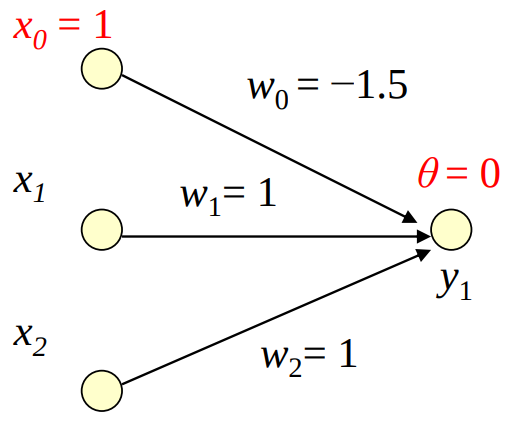
\includegraphics[width=0.9\linewidth]{images/lecture-perceptron.png}
    \end{minipage}
    \begin{minipage}[h]{0.4\linewidth}
        \begin{tabularx}{0.8\textwidth}{>{\centering\arraybackslash}X>{\centering\arraybackslash}X|>{\centering\arraybackslash}X>{\centering\arraybackslash}X}
            \hline
            $x_1$ & $x_2$ & net & out \\
            \hline
            0 & 0 & \textbf{-1.5} & \textbf{0}\\
            \hline
            0 & 1 & \textbf{-0.5} & \textbf{0}\\
            \hline
            1 & 0 & \textbf{-0.5} & \textbf{0}\\
            \hline
            1 & 1 & \textbf{0.5} & \textbf{1}\\
            \hline
        \end{tabularx}
    \end{minipage}
    \caption{2차원 입력을 받는 AND Gate를 구현한 1층 퍼셉트론의 모습. $x_0=1$로 고정되어있는데, 이는 $w_0$가 bias의 역할을 한다는 것을 의미한다. 그리고 $\theta=0$ 이라는 것은 퍼셉트론의 입력 벡터에 가중치 벡터를 내적하여 나온 값(net)이 0 보다 클 때 모델의 출력을 1로, 그렇지 않으면 0으로 하겠다는 것을 의미한다.}
\end{figure}

수업에서는 2개의 boolean values가 주어지는 상황에서 AND, OR 등의 논리 연산을 어떻게 구현할 수 있을지를 생각하였다. 그런데 현실에서는 2개의 입력에 대한 AND 뿐만이 아니라 $n$개의 입력에 대한 AND Gate 또한 생각할 수 있다. $(n\geq 2)$

2차원 벡터를 입력으로 받는 AND Perceptron을 $n$차원 벡터를 입력으로 받는 AND Perceptron으로 확장해보자. 이 퍼셉트론은 입력으로 $n$차원 벡터 $(x_1, x_2, \dots, x_n)$가 주어지고, 퍼셉트론의 가중치가 $(w_0, w_1, w_2, \dots, w_n)$ (단, $w_0$는 bias)일 때, 퍼셉트론의 출력 out이 아래와 같이 결정될 것이다.

\[
\textbf{net}=w_0 + \sum_{i=1}^{n} x_i w_i, \textbf{ out}=\left.
\begin{cases}
    1, & \text{if }net > 0\\
    0, & \text{otherwise.}
\end{cases}
\right\}
\]

이 과제물에서는 위와 같이 $n$차원으로 일반화한 AND Perceptron을 시뮬레이팅하는 프로그램을 C++로 구현하고, 올바른 출력을 내는 $n$차원 AND Perceptron을 생성하려면 가중치를 어떻게 설정해야 하는지를 논의한다.

\section{C++을 이용한 퍼셉트론의 구현}

C++로 구현한 전체 코드는 이 보고서와 함께 첨부된 소스파일을 통해 확인할 수 있다.

\begin{itemize}
    \item \textbf{Perceptron.h}: $n$차원 벡터에 대하여 AND 논리 연산을 계산하는 \texttt{Perceptron} 클래스를 선언한 헤더파일
    \item \textbf{Perceptron.cpp}: Perceptron.h에서 선언한 메서드의 본문을 정의한 소스파일
    \item \textbf{Main.cpp}: \texttt{main} 함수에서 퍼셉트론을 시뮬레이팅하는 소스파일
    \item \textbf{Makefile}: 소스 빌드 방법을 정의한 Makefile. \textbf{build-essential} 패키지가 설치된 Linux 환경에서 '\texttt{make}' 명령어를 이용하여 빌드할 수 있음.
\end{itemize}

소스코드의 주요 부분에 주석을 삽입해두었으므로, 이 보고서에서는 \texttt{Perceptron} 클래스의 동작 방식과 \texttt{main} 함수의 역할을 서술한다.

\subsection{Perceptron 클래스}

Perceptron.h와 Perceptron.cpp 파일에서 정의하고 있는 \texttt{Perceptron} 클래스는 $n$차원 boolean vector를 입력으로 하였을 때 아래 식에 따라 퍼셉트론의 출력을 계산하는 클래스이다.

\[
f(x_1, x_2, \dots, x_n)=\left.
\begin{cases}
    1, & \text{if }w_0 + \sum_{i=1}^{n} x_i w_i > 0\\
    0, & \text{otherwise.}
\end{cases}
\right\}
\]

실제 코드상에서는 퍼셉트론의 Bias를 뜻하는 $w_0$가 멤버 변수 \texttt{bias}에 저장되고, 그 외 가중치 $w_1, w_2, \dots, w_n$는 멤버변수 \texttt{weights}에 저장된다. 객체를 처음 생성하면 Bias와 모든 가중치가 $[-1, 1]$ 내의 임의의 실수 값으로 초기화된다. 이는 필요시 추후에 public methods를 이용하여 손쉽게 업데이트할 수 있다.

그리고 특정 $n$차원 입력 벡터에 대하여 출력값을 계산할 때는 입력으로 들어온 $bool$형 변수가 참일 경우에 1, 그렇지 않으면 0이라고 가정하고 위에서 소개한 수식을 통해 출력값을 계산한다.

\subsection{main 함수의 동작 과정}

Main.cpp에 정의된 \texttt{main} 함수는 과제 명세서에서 정의된 과정을 그대로 구현하고 있다.

\begin{enumerate}
    \item 사용자로부터 Input 차원의 크기를 입력받고, 그 크기에 맞게 AND Perceptron을 생성한다.
    \item \texttt{Perceptron}의 생성자에서 퍼셉트론의 bias와 weights가 모두 $[-1, 1]$ 내의 임의의 실수 값으로 초기화된다.
    \item \texttt{checkOutputs} 함수의 반환값이 거짓일 동안 사용자로부터 새로운 가중치 값을 입력 받고 그 값으로 가중치를 갱신한다. \texttt{checkOutputs}는 각 input에 대한 output을 모두 확인하고 진리표와 맞은 개수를 출력한 뒤, 모든 input에 대하여 올바른 결과가 나타났을 때 참, 그렇지 않으면 거짓을 반환한다.
\end{enumerate}

사용자가 퍼셉트론의 가중치를 올바르게 설정하지 않는다면 프로그램이 계속해서 무한 루프를 실행하게 되므로, 사용자가 퍼셉트론의 올바른 가중치를 빨리 입력할수록 프로그램이 일찍 종료하게 된다.

\section{가중치를 올바르게 설정하는 방법}

이제 $n$차원 입력을 받는 AND Perceptron의 가중치(bias 포함)가 어떻게 설정되어야 퍼셉트론이 올바른 출력을 내게 되는지를 논의한다.

AND Gate의 특성을 다시 한번 생각해보면, 입력되는 $n$ $(n\geq 2)$차원 벡터가 모두 참이어야 출력이 참이고, 단 하나라도 거짓인 입력이 존재한다면 출력이 거짓이다. 즉 가중치를 나타내는 벡터 $(w_0, w_1, \dots, w_n)$가 아래 두 조건을 만족할 때 퍼셉트론의 출력이 모두 올바를 것이다. (단, 임의의 $x_i$는 0 또는 1 이다.)

\begin{enumerate}
    \item $1\leq i \leq n$를 만족하는 \textbf{모든 정수} $i$에 대하여 $x_i=1$ 이면 $w_0 + \sum_{i=1}^{n} x_i w_i > 0$이다.
    \item $1\leq i \leq n$를 만족하는 \textbf{어떤 정수} $i$에 대하여 $x_i=0$ 이면 $w_0 + \sum_{i=1}^{n} x_i w_i < 0$이다.
\end{enumerate}

위 두 조건을 만족하는 가중치 벡터는 무한함이 자명하므로, 가중치를 올바르게 설정하는 방법은 수없이 많을 것이다. 위 조건을 만족하는 한 가지 예로 아래와 같이 설정된 가중치 벡터를 들 수 있다. 아래와 같이 가중치를 설정할 경우 \textbf{퍼셉트론이 올바른 AND Gate를 구성하게 되므로 loop에서 곧바로 탈출할 수 있다.}

입력 벡터의 차원의 수가 $n$ $(n\geq 2)$일 때,
\begin{itemize}
    \item $w_0=\frac{1}{2}-n$
    \item $w_i=1$ $(1\leq i \leq n)$
\end{itemize}

\subsection{위 방법이 유효하다는 증명}

위 방법과 같이 가중치를 할당할 경우, 퍼셉트론에서 합산한 결과는 아래와 같게 된다.

\[
\textbf{net}=\frac{1}{2}-n+\sum_{i=1}^{n} x_i
\]

\begin{enumerate}
    \item $1\leq i \leq n$를 만족하는 \textbf{모든 정수} $i$에 대하여 $x_i=1$ 일 경우, \\
    \begin{align*}
        \textbf{net} &=\frac{1}{2}-n+\sum_{i=1}^{n} x_i \\
        &=\frac{1}{2}-n+n \\
        &=\frac{1}{2} > 0
    \end{align*}
    따라서 이 경우 퍼셉트론은 1을 출력값으로 반환한다.
    
    \item $1\leq i \leq n$를 만족하는 \textbf{어떤 정수} $i$에 대하여 $x_i=0$ 일 경우, $\sum_{i=1}^{n} x_i \leq n-1$이므로, 양변에 $\frac{1}{2}-n$를 더하면 \\
    \begin{align*}
        \frac{1}{2}-n+\sum_{i=1}^{n} x_i \leq -\frac{1}{2} < 0 \\
    \end{align*}
    따라서 이 경우 퍼셉트론은 0을 출력값으로 반환한다.
    
\end{enumerate}

위 두 경우에 따른 출력값이 AND Gate의 출력 양상과 같으므로, 이 방법으로 가중치를 할당하면 올바른 AND Gate를 구성할 수 있다. (loop에서 곧바로 탈출할 수 있다.)

\subsection{실행 예시 $(n=2)$}

아래 실행 예시는 $n=2$로 설정하고 무작위로 설정한 가중치가 틀렸을 때, $w_0=-1.5$, $w_1=1$, $w_2=1$를 입력하여 바로 루프를 탈출하는 모습이다.

\begin{minted}
[
frame=lines,
framesep=2mm,
baselinestretch=1.2,
fontsize=\footnotesize,
linenos
]
{text}
Enter input dimensions of AND Gate: 2
Generated perceptron with random bias and weights!

   < 1st Truth Table >    
   x1   |   x2   | Output 
--------------------------
   0    |   0    |   0    
   1    |   0    |   0    
   0    |   1    |   1    
   1    |   1    |   1    
Count of Correct Outputs = 3

Some outputs are wrong.
You MUST update bias and weights.

Update bias(w0): -1.5
Update w1: 1
Update w2: 1

   < 2nd Truth Table >    
   x1   |   x2   | Output 
--------------------------
   0    |   0    |   0    
   1    |   0    |   0    
   0    |   1    |   0    
   1    |   1    |   1    
Count of Correct Outputs = 4

Finally all outputs are CORRECT!
\end{minted}

\subsection{실행 예시 $(n=4)$}

아래 실행 예시는 $n=4$로 설정하고 무작위로 설정한 가중치가 틀렸을 때, $w_0=-3.5$, $w_1=1$, $w_2=1$, $w_3=1$, $w_4=1$를 입력하여 바로 루프를 탈출하는 모습이다.

\begin{minted}
[
frame=lines,
framesep=2mm,
baselinestretch=1.2,
fontsize=\footnotesize,
linenos
]
{text}
Enter input dimensions of AND Gate: 4
Generated perceptron with random bias and weights!

            < 1st Truth Table >             
   x1   |   x2   |   x3   |   x4   | Output 
--------------------------------------------
   0    |   0    |   0    |   0    |   1    
   1    |   0    |   0    |   0    |   1    
   0    |   1    |   0    |   0    |   1    
   1    |   1    |   0    |   0    |   1    
   0    |   0    |   1    |   0    |   1    
   1    |   0    |   1    |   0    |   1    
   0    |   1    |   1    |   0    |   1    
   1    |   1    |   1    |   0    |   1    
   0    |   0    |   0    |   1    |   0    
   1    |   0    |   0    |   1    |   0    
   0    |   1    |   0    |   1    |   0    
   1    |   1    |   0    |   1    |   0    
   0    |   0    |   1    |   1    |   0    
   1    |   0    |   1    |   1    |   0    
   0    |   1    |   1    |   1    |   0    
   1    |   1    |   1    |   1    |   0    
Count of Correct Outputs = 7

Some outputs are wrong.
You MUST update bias and weights.

Update bias(w0): -3.5
Update w1: 1
Update w2: 1
Update w3: 1
Update w4: 1

            < 2nd Truth Table >             
   x1   |   x2   |   x3   |   x4   | Output 
--------------------------------------------
   0    |   0    |   0    |   0    |   0    
   1    |   0    |   0    |   0    |   0    
   0    |   1    |   0    |   0    |   0    
   1    |   1    |   0    |   0    |   0    
   0    |   0    |   1    |   0    |   0    
   1    |   0    |   1    |   0    |   0    
   0    |   1    |   1    |   0    |   0    
   1    |   1    |   1    |   0    |   0    
   0    |   0    |   0    |   1    |   0    
   1    |   0    |   0    |   1    |   0    
   0    |   1    |   0    |   1    |   0    
   1    |   1    |   0    |   1    |   0    
   0    |   0    |   1    |   1    |   0    
   1    |   0    |   1    |   1    |   0    
   0    |   1    |   1    |   1    |   0    
   1    |   1    |   1    |   1    |   1    
Count of Correct Outputs = 16

Finally all outputs are CORRECT!
\end{minted}

\end{document}
